\documentclass[conference]{IEEEtran}

\usepackage{hyperref}
\usepackage{tikz}
\usetikzlibrary{shapes.geometric, arrows}

\title{AI Infrastructure Design for Automated Lunar and Martian Crater Detection}

\author{
	\IEEEauthorblockN{Scott Nguyen}
	\IEEEauthorblockA{
		University of New Mexico \\
		snguyen9@unm.edu
	}
}

\begin{document}
	
	\maketitle
	
	\begin{abstract}
		This paper presents a cloud-based AI infrastructure design for automated detection of lunar and Martian craters from satellite imagery. The system leverages deep learning models such as YOLOv8 and U-Net to identify crater locations and boundaries at scale. The infrastructure is built on Amazon Web Services (AWS) using GPU-accelerated compute, scalable storage, managed databases, and auto-scaling to handle large datasets efficiently. The design emphasizes scalability, reliability, security, and cost efficiency while supporting future growth and integration with additional space mission datasets.
	\end{abstract}
	
	\begin{IEEEkeywords}
		AI Infrastructure, Computer Vision, Crater Detection, AWS, EC2, S3, RDS, Auto Scaling, YOLOv8, U-Net, NVIDIA A100
	\end{IEEEkeywords}
	
	\section{Introduction}
	
	Planetary exploration generates large amounts of image data captured by orbiters and landers. Identifying craters within this data is important for terrain analysis, surface geology research, and future landing site selection. Manual analysis is slow and difficult to scale, making automated computer vision systems an attractive solution.
	
	This project focuses on designing the infrastructure needed to support an AI-based crater detection pipeline rather than building the model itself. The proposed system uses Amazon Web Services (AWS) to provide scalable compute, storage, and database resources for efficient processing and analysis.
	
	\subsection{Motivation}
	
	Modern planetary missions generate massive amounts of imagery from orbiters, rovers, and landers. As missions continue to increase in scale, manually analyzing these datasets becomes increasingly difficult and time consuming. Automated crater detection systems can help researchers process data more efficiently while improving consistency and scalability.
	
	Crater identification is also important for multiple mission objectives beyond surface analysis. Crater density can provide insight into planetary age and geological history, while terrain analysis can support hazard assessment and landing site selection. As a result, scalable AI infrastructure has become increasingly relevant for future space exploration workflows.
	
	\section{Requirements Analysis}
	
	The system requirements are driven by the need to process large, high-resolution planetary images using deep learning models.
	
	\subsection{Compute Requirements}
	
	GPU acceleration is required for efficient model inference and training. Deep learning models such as YOLOv8 and U-Net rely heavily on parallel computation, making GPU-based infrastructure significantly faster than CPU-only systems. CPUs are still necessary for preprocessing, orchestration, and data management.
	
	\subsection{Storage Requirements}
	
	The system must store raw satellite imagery, processed images, trained model files, and crater detection outputs. Since this data is unstructured and large-scale, object storage is the most appropriate solution.
	
	\subsection{Database Requirements}
	
	Structured outputs such as crater coordinates and metadata require a relational database for querying and long-term storage.
	
	\subsection{Networking Requirements}
	
	Data must move efficiently between storage, compute, and user-facing APIs. While the system is not strictly real-time, reliable networking is still important for maintaining throughput.
	
	\subsection{Software Requirements}
	
	The software stack includes:
	\begin{itemize}
		\item Python
		\item PyTorch
		\item OpenCV
		\item Docker
	\end{itemize}
	
	These tools provide flexibility for AI model deployment and image processing.
	
	\section{Infrastructure Design}
	
	The infrastructure is fully cloud-based using Amazon Web Services (AWS).
	
	\subsection{System Architecture Overview}
	
	\begin{figure}[ht]
		\centering
		
		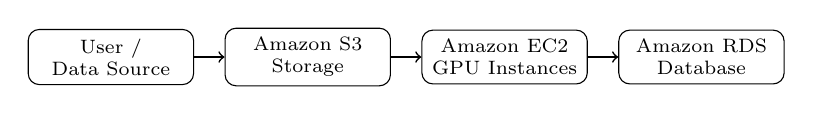
\begin{tikzpicture}[
			box/.style={
				rectangle,
				draw,
				rounded corners,
				minimum width=2.1cm,
				minimum height=0.65cm,
				align=center,
				font=\scriptsize
			},
			arrow/.style={
				->,
				line width=0.6pt
			}
			]
			
			\node (user) [box] at (0,0) {User /\\Data Source};
			\node (s3) [box] at (2.5,0) {Amazon S3\\Storage};
			\node (ec2) [box] at (5.0,0) {Amazon EC2\\GPU Instances};
			\node (rds) [box] at (7.5,0) {Amazon RDS\\Database};
			
			\draw [arrow] (user) -- (s3);
			\draw [arrow] (s3) -- (ec2);
			\draw [arrow] (ec2) -- (rds);
			
		\end{tikzpicture}
		
		\vspace{-2mm}
		\caption{High-level architecture of the crater detection system}
		\vspace{-4mm}
		
	\end{figure}
	
	\subsection{Compute Infrastructure}
	
	Amazon EC2 provides scalable virtual servers with multiple instance categories optimized for different workloads.
	
	These include:
	\begin{itemize}
		\item General-purpose instances
		\item Compute-optimized instances
		\item Memory-optimized instances
		\item Accelerated computing instances
		\item Storage-optimized instances
		\item HPC-optimized instances
	\end{itemize}
	
	For this project, accelerated computing instances are selected because they include GPUs suitable for deep learning workloads.
	
	The NVIDIA A100 GPU is chosen due to its strong performance for AI training and inference. The A100 supports large-scale datasets, high memory bandwidth, and efficient parallel processing.
	
	\subsection{AI Model Selection}
	
	Two primary model architectures are considered in this project: YOLOv8 and U-Net.
	
	YOLOv8 is an object detection model optimized for fast inference and real-time performance. It can identify crater locations using bounding boxes and is well suited for efficiently processing large datasets.
	
	U-Net is a segmentation-based architecture that performs pixel-level classification. Unlike object detection models, segmentation models can identify crater boundaries more precisely, which may improve scientific analysis at the expense of additional computational cost.
	
	The infrastructure is designed to support either approach depending on mission requirements and desired output accuracy.
	
	\subsection{Storage Infrastructure}
	
	Amazon S3 is used for storing all image data. S3 provides industry-leading scalability, durability, and availability, making it ideal for large-scale AI workloads and image datasets.
	
	\subsection{Database Infrastructure}
	
	Amazon RDS stores structured outputs such as crater locations and metadata. RDS automates provisioning, backups, and scaling while maintaining high availability.
	
	\subsection{Infrastructure Components}
	
	\begin{table}[ht]
		\centering
		\caption{Infrastructure Components and Roles}
		\begin{tabular}{|p{0.22\linewidth}|p{0.28\linewidth}|p{0.36\linewidth}|}
			\hline
			\textbf{Component} & \textbf{Service} & \textbf{Purpose} \\ \hline
			Compute & EC2 GPU instances & Run AI models \\ \hline
			Storage & Amazon S3 & Store images and datasets \\ \hline
			Database & Amazon RDS & Store crater results \\ \hline
			Scaling & AWS Auto Scaling & Adjust resources dynamically \\ \hline
			AI Model & YOLOv8 or U-Net & Detect craters in images \\ \hline
		\end{tabular}
	\end{table}
	
	\section{Scalability and Reliability}
	
	Scalability is achieved using AWS Auto Scaling, which automatically adjusts compute resources depending on workload demand.
	
	\begin{figure}[ht]
		\centering
		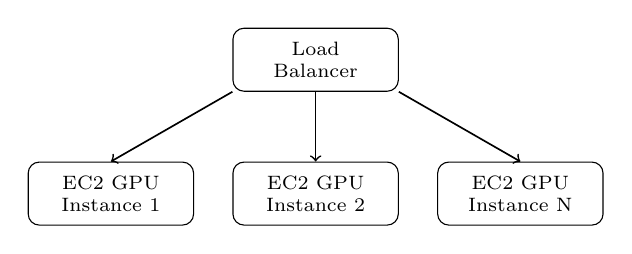
\begin{tikzpicture}[
			box/.style={
				rectangle,
				draw,
				rounded corners,
				minimum width=2.1cm,
				minimum height=0.8cm,
				align=center,
				font=\scriptsize
			},
			arrow/.style={->, line width=0.6pt}
			]
			
			\node (lb) [box] at (0,0) {Load\\Balancer};
			
			\node (ec21) [box] at (-2.6,-1.7) {EC2 GPU\\Instance 1};
			\node (ec22) [box] at (0,-1.7) {EC2 GPU\\Instance 2};
			\node (ec23) [box] at (2.6,-1.7) {EC2 GPU\\Instance N};
			
			\draw [arrow] (lb.south west) -- (ec21.north);
			\draw [arrow] (lb.south) -- (ec22.north);
			\draw [arrow] (lb.south east) -- (ec23.north);
			
		\end{tikzpicture}
		
		\vspace{-2mm}
		\caption{Auto-scaling and load balancing of compute resources}
		\vspace{-4mm}
	\end{figure}
	
	As image workloads increase, additional EC2 GPU instances can automatically be launched to maintain performance. This makes the design useful for both small research workloads and larger mission-scale datasets.
	
	Reliability is maintained through redundancy and managed cloud services. Amazon S3 provides highly durable storage, while Amazon RDS supports multi-zone deployments to reduce the risk of data loss.
	
	Another reliability benefit is that the system separates storage, compute, and database responsibilities. If a compute instance fails during processing, the original imagery remains stored in S3 and the job can be retried on another instance. This prevents one failed compute node from causing permanent data loss.
	
	\section{Security and Privacy}
	
	Security is implemented using AWS cloud security features. Data is encrypted both at rest and in transit.
	
	Identity and access management (IAM) policies are used to control access to system resources. AWS also provides monitoring, compliance, and logging tools that help maintain infrastructure security.
	
	These security measures ensure that mission data and processed outputs remain protected while still allowing authorized access.
	
	\subsection{Future Improvements}
	
	Future improvements to the system could include support for real-time satellite data ingestion, distributed multi-GPU training, and integration with additional planetary datasets. More advanced orchestration tools such as Kubernetes could also be introduced to further automate deployment and scaling.
	
	Another potential improvement would involve integrating model retraining pipelines that continuously improve crater detection accuracy as new labeled datasets become available. This would allow the infrastructure to support not only inference, but also long-term model improvement over time.
	
	\section{Cost Estimation and Comparison}
	
	The primary cost drivers of the system are compute, storage, and networking.
	
	GPU-based EC2 instances are the most expensive component because they are billed hourly. However, GPU acceleration significantly improves model inference speed and overall processing throughput.
	
	Storage costs from Amazon S3 are relatively low and scale with the size of the dataset. RDS pricing depends on database instance type and usage.
	
	An alternative approach is to use Amazon Bedrock, which charges per token processed. Some models cost approximately \$0.20--\$2.00 per million input tokens, with higher output token costs.
	
	For this specific crater detection system, the self-hosted EC2 approach is more appropriate because the workload is image-based and requires control over computer vision models. Managed generative AI services are useful for text and multimodal applications, but they do not provide the same level of control over model training, image preprocessing, and crater-specific output formatting.
	
	\begin{table}[ht]
		\centering
		\caption{Self-Hosted vs Managed AI Comparison}
		\begin{tabular}{|p{0.25\linewidth}|p{0.30\linewidth}|p{0.30\linewidth}|}
			\hline
			\textbf{Category} & \textbf{EC2 GPU System} & \textbf{Amazon Bedrock} \\ \hline
			Cost Model & Hourly GPU billing & Pay per token \\ \hline
			Scalability & Uses Auto Scaling & Fully managed \\ \hline
			Control & Full model control & Limited model control \\ \hline
			Complexity & Higher setup effort & Lower setup effort \\ \hline
			Best Use & Large image datasets & Smaller AI workloads \\ \hline
		\end{tabular}
	\end{table}
	
	\subsection{Example Monthly Cost Estimate}
	
	\begin{table}[ht]
		\centering
		\caption{Example Monthly Cost Estimate}
		\begin{tabular}{|p{0.28\linewidth}|p{0.28\linewidth}|p{0.22\linewidth}|}
			\hline
			\textbf{Component} & \textbf{Configuration} & \textbf{Estimated Cost} \\ \hline
			EC2 GPU Instance & A100 GPU instance & \$1200--\$1500 \\ \hline
			Amazon S3 & 10 TB storage & \$200--\$300 \\ \hline
			Amazon RDS & db.r6g.large & \$150--\$250 \\ \hline
			Networking & Data transfer & \$50--\$100 \\ \hline
			Total & Approximate monthly cost & \$1600--\$2150 \\ \hline
		\end{tabular}
	\end{table}
	
	The cost estimate is intended as an approximate planning value rather than a fixed final price. Actual cost would depend on the number of images processed, GPU runtime, storage volume, and data transfer. For a course-scale or research prototype, the system could be run only when needed to reduce GPU costs. For a production-scale mission archive, the system would likely require a larger and more continuous compute budget.
	
	\section{Conclusion}
	
	This paper presented a cloud-based AI infrastructure for automated lunar and Martian crater detection. The proposed design leverages GPU-accelerated compute, scalable storage, managed databases, and auto-scaling to efficiently process large planetary image datasets.
	
	By balancing performance, scalability, reliability, security, and cost, the system provides a practical solution for future space-related AI applications and demonstrates how cloud infrastructure can support modern computer vision workloads in planetary science.
	
	\subsection{Potential Research Applications}
	
	Beyond crater detection, the proposed infrastructure could support additional planetary science applications involving large-scale image analysis. Similar computer vision pipelines could be adapted for dust storm tracking on Mars, rock and terrain classification, or identifying geological features from orbital imagery. Because the infrastructure is cloud-based and modular, new models and datasets could be integrated without requiring major architectural changes.
	
	The infrastructure could also support collaborative scientific workflows. Researchers from different institutions could upload datasets, run inference jobs, and access processed outputs through centralized APIs and cloud storage. This would simplify data sharing and improve reproducibility across research teams.
	
	Another important advantage of the proposed architecture is flexibility. Different EC2 instance types and GPU configurations can be selected depending on mission scale and computational demand. Smaller research projects may only require a single GPU instance, while larger mission archives could distribute workloads across multiple auto-scaled compute nodes.
	
	Overall, the proposed design demonstrates how modern cloud infrastructure can support scalable AI workflows for future planetary exploration missions while remaining flexible enough for evolving research needs.
	
	\begin{thebibliography}{00}
		
		\bibitem{ec2}
		Amazon EC2. Available: \url{https://aws.amazon.com/ec2/}
		
		\bibitem{s3}
		Amazon S3. Available: \url{https://aws.amazon.com/s3/}
		
		\bibitem{rds}
		Amazon RDS. Available: \url{https://aws.amazon.com/rds/}
		
		\bibitem{autoscaling}
		AWS Auto Scaling. Available: \url{https://aws.amazon.com/autoscaling/}
		
		\bibitem{security}
		AWS Security. Available: \url{https://aws.amazon.com/security/}
		
		\bibitem{bedrock}
		Amazon Bedrock Pricing. Available: \url{https://aws.amazon.com/bedrock/pricing/}
		
		\bibitem{a100}
		NVIDIA A100 GPU. Available: \url{https://www.nvidia.com/en-us/data-center/a100/}
		
		\bibitem{yolo}
		Ultralytics YOLOv8 Documentation. Available: \url{https://docs.ultralytics.com/models/yolov8/}
		
		\bibitem{unet}
		Ultralytics U-Net Guide. Available: \url{https://www.ultralytics.com/blog/a-guide-on-u-net-architecture-and-its-applications}
		
	\end{thebibliography}
	
\end{document}